
\chapter{Metodologia Proposta} \label{met}

% esse é o texto introdutório. Ele tem que servir como um bom resumo do que o capítulo oferece, de modo que mesmo que a pessoa só leia a introdução ela já tenha uma boa noção do que se trata.
%\textcolor{red}{Felipe, nao dah para comecar uma secao jogando na cara do leitor o que o metodo faz... Aqui voce deve colocar um ou dois paragrafos falando que o metodo foi organizado de modo a detectar bordas de tv em imagens, as quais sao tratadas como objetos quadrangulares. Estes, por sua vez, sao definidos por quatro lados, ou seja, linhas. Sendo assim, determinou-se, com base no algoritmo de fulano de tal (aquela ref dos japoneses), que isso seria feito em quatro passos: detecção de bordas, pois as linhas da tela sao nada mais, nada menos que a bordas entre o quadro e a tela, identificação das linhas, com o objetivo de reconhecer componentes conectados, reconhecimento de retangulos, para que linhas formando retangulos sejam separadas, e escolha do retangulo, que deve atender a certos critérios, como relacao de aspecto de 4:3 ou 16:9... Entendeu? Coloque uns dois paragrafos sobre isso e essas explicações rápidas que eu coloquei, sobre cada passo, devem ser melhoradas e colocadas ao lado de cada item na lista (itemize). Ao final, fale que cada passo serah detalhado nas proximas secoes...}

%Este capítulo apresenta o método de detecção e extração de tela de TV de uma imagem, assim como as técnicas para verificar a corretude da extração. O problema detecção da tela de TV é encarado como um subtipo da detecção de objetos quadrangulares, já que as quatro bordas do monitor são encaradas como linhas que formam um objeto quadrangular.

%Partindo desta definição, foi montado um método com base no algoritmo proposto por Liu, Ikenaga e Goto \cite{mrf}. Este método é dividido em quatro etapas, que são como segue:

\textcolor{red}{Este capítulo apresenta o método de detecção e extração de telas de TV e monitores, bem como as métricas de desempenho utilizadas para avaliar o método. Ele está organizado em seções, que são como segue: a introdução contextualiza o problema de detecção de objetos quadrangulares e telas de TV e monitores, a Detecção de Bordas aborda as técnicas utilizadas neste método para detectar bordas, a Detecção de Linhas detalha como foi feita a detecção de linhas, o Reconhecimento de Retângulos aborda as técnicas utilizadas para reconhecer as linhas encontradas como parte de retângulos, assim como o processo de escolha do retângulo que representa a tela.}

\section{Introdução}

O problema da detecção de objetos quadrangulares em imagens \cite{quadquadrinhos ,objquadrangular00} possui diversas aplicações. Por exemplo, navegação de robôs \cite{navegrobo,navegrobo00} e detecção de prédios em imagens de satélites \cite{prediosatelite,prediosatelite00,prediosatelite01}. % e de placas que indicam material perigoso \cite{materialperig}. http://ieeexplore.ieee.org/xpls/icp.jsp?arnumber=1048435&tag=1
 Para caracterizarmos o problema da detecção de objetos quadrangulares precisamos considerar que um objeto quadrangular \cite{quadquadrinhos} em uma imagem é definido como um objeto delimitado por quatro segmentos de reta distintos pertencentes à imagem, conectados por quatro vértices. Em particular, podemos encarar a detecção de telas de TV e monitores como um problema de detecção de objetos quadrangulares \cite{inspect}. De fato, isto pode ser feito devido à padronização da fabricação de TVs e monitores \cite{DVB}, que recomenda algumas características para as telas. Este cenário favorece a criação de um sistema de inspeção de telas podendo auxiliar sistemas para inspeção automática \cite{inspect}.

%importancia detecção de telas de tv
%A importância deste método está na sua utilização para inspeção automática de TVs. Sistemas de inspeção automática de TVs recentes capturam a imagem a ser mostrada na tela \cite{inspectgrabber}, antes de ela ser mostrada, para compará-la com uma imagem de referência. Esta técnica, embora rápida, não detecta problemas na tela do ponto de vista do usuário. Utilizando o método aqui proposto, é possível detectar quando a imagem na memória da TV ou monitor não corresponde à imagem mostrada na tela ou quando a operação da TV tem algum problema.
%Sistemas de inspeção automática de TVs recentes capturam a imagem a ser mostrada na tela \cite{inspectgrabber}, antes de ela ser mostrada, para compará-la com uma imagem de referência. Esta técnica, embora rápida, não detecta problemas na tela do ponto de vista do usuário. %elaborar mais

%Inúmeros trabalhos foram desenvolvidos envolvendo inspeção automática de TVs. Como por exemplo, existem trabalhos focados em encontrar erros no software utilizado no aparelho, tais como \textit{deadlocks}, vazamentos de memória e problemas na alocação de tarefas \cite{inspectsoftware}. Há trabalhos focados em encontrar problemas na interação entre hardware e software \cite{inspecthardsoft}, e ainda outros focados na análise da qualidade da imagem mostrada \cite{inspectimage00,inspectimage01,inspectimage02}. Trabalhos mais recentes têm focado em uma análise dos http://servicos.netcombo.com.br/netPortalWEB/appmanager/portal/desktop?_nfpb=true&_pageLabel=cadastro_page&bew=1erros de operação nos aparelhos de TV \cite{inspectgrabber}.

PARÁGRAFO PARA A INTRODUÇÃO

A detecção de falhas em TVs e monitores é um problema abordado por diversos trabalhos e alguns destes utilizam técnicas de campos multidisciplinares, como processamento de sinais, engenharia de software, IA e RP. Por exemplo, no sistema mostrado em \cite{inspectsoftware}, os autores propõem encontrar erros no software utilizado no aparelho, tais como \textit{deadlocks}, vazamentos de memória e problemas na alocação de tarefas \textcolor{red}{explicar mais}. Outro exemplo é apresentado em \cite{inspecthardsoft}, que usa um sinal de referência misturado com um sinal de erro através de software para encontrar problemas na interação entre hardware e software. Alguns trabalhs de detecção de falhas propõem um sistema de inspeção automática baseado na análise digital da imagem mostrada, técnica que permite verificar tanto hardware quanto software \cite{inspect,inspectimage00,inspectimage01,inspectimage02,inspectgrabber} \textcolor{red}{explicar mais}.

Os métodos de inspeção automática de TVs e monitores por análise digital da imagem podem ser divididos em duas categorias principais. Na primeira, encontramos os métodos em que a captura da imagem é feita diretamente da memória da TV ou monitor. Perceba que a captura é feita antes da exibição da imagem na TV ou monitor \cite{inspectimage00,inspectimage03,inspectimage04}. Esta categoria de métodos proporciona a detecção de erros de hardware e software que produzam como resultado uma imagem defeituosa na memória da TV ou monitor. Na segunda, temos os métodos em que a captura da imagem é feita através de uma câmera \cite{inspect,vantagemauto}. Assim, podemos analisar a imagem exibida na TV ou monitor do ponto de vista do usuário.
 conseguimos detectar, além das falhas detectadas na primeira categoria, problemas nos circuitos entre a memória interna da TV e a tela.
%A importância deste método está na sua utilização para inspeção automática de TVs. Utilizando o método aqui proposto, é possível detectar quando a imagem na memória da TV ou monitor não corresponde à imagem mostrada na tela ou quando a operação da TV tem algum problema. %refazer essa frase toda. dados.

Geralmente, os métodos de inspeção automática de TVs e monitores em que a captura da imagem é feita por uma câmera utilizam uma ou mais das seguintes etapas:

\begin{itemize}
\item \textbf{pré-processamento}: as imagens capturadas geralmente necessitam de algum pré-processamento, seja para eliminar ruído ou para destacar as características necessárias para que as etapas seguintes possam ser executadas.
\item \textbf{detecção da região da tela na imagem}: utilizando as informações geradas na fase de pré-processamento, o método deve ser capaz de identificar na imagem a região que corresponde  à tela. Isto normalmente é feito através de uma combinação de detecção de retângulos e identificação, se aproveitando de características da tela.
\item \textbf{extração do conteúdo da tela}: identificada a região, nesta etapa é feita a extração do conteudo da tela. Ele é extraído para um formato que seja compatível com a etapa de comparação.
\item \textbf{inspeção}: nesta etapa é feita a inspeção a tela, através da comparação do conteúdo extraído com uma ou mais referências. A comparação pode ser feita de diversas formas, utilizando toda a imagem capturada ou parte dela. O resultado pode ser uma pontuação, uma imagem ou um rótulo (ok ou não ok).
\end{itemize}

Nesta dissertação, conforme comentamos, apresentamos um método de detecção de telas que representa uma alternativa para integrar um sistema de inspeção automática de telas de TV e monitores. \textcolor{red}{inserir vantagens, motivações e contribuições aqui}. Uma contribuição deste trabalho é aliar o método de detecção de tela às técnicas de detecção de borda através de análise de gradiente multi-dimensional e detecção de retângulo utilizando um modelo baseado no Campo Aleatório de Markov, apresentadas em \cite{mrf}.

%O método proposto apresenta uma alternativa de inspeção automática de TVs e monitores, adquirindo o conteúdo da tela através de uma câmera fotográfica e comparando este conteúdo com imagens de referência. Este curso de ação apresenta a vantagem de conseguir analisar a imagem do ponto de vista do usuário final, além de poder verificar problemas no circuito entre a tela e a memória da TV ou monitor e problemas na funcionalidade da TV \cite{inspect}.

\begin{comment}


%nao eh trivial, pois envolve diversos metodos de processamrto

Este não é um problema de solução trivial. A resolução deste problema envolve diversos métodos de processamento digital de imagens, tais como detecção de telas, detecção de linhas, mesclagem de linhas, classificação de linhas e detecção de objetos retangulares.

%A fim de gerar uma alternativa de solução para o problema da detecção de telas de TV e monitores,
%comentar mais sobre as etapas utilizadas
%foi criado um método com base no algoritmo proposto em \cite{mrf}. Este método é dividido em quatro etapas, que são como segue:
A fim de gerar uma alternativa de solução para o problema da detecção de telas de TV e monitores,
%comentar mais sobre as etapas utilizadas
foi criado um método com base no algoritmo proposto em \cite{mrf}. A ideia basica deste método é classificar as linhas presentes na imagem como lados de um objeto retangular através de um modelo MRF e após isto identificar o objeto que representa a tela. Este método é dividido em quatro etapas, que são como segue:

%\end{comment}

%O método é baseado no algoritmo proposto em \cite{mrf}. A ideia básica deste método é classificar as linhas presentes na imagem como lados de um objeto retangular através de um modelo MRF e, após isto, identificar o objeto que representa a tela. É uma operação que envolve diversos métodos de processamento digital de imagens, tais como detecção de telas, detecção de linhas, mesclagem de linhas, classificação de linhas e detecção de objetos retangulares. Este método é dividido em quatro etapas, que são como segue:

O método aqui apresentado consiste nas seguintes etapas, que serão detalhados nas seções seguintes: \textcolor{red}{se vou apresentar nas próximas seções, pq fazer um resumo em bullet points agora?}

\begin{itemize}
%porque usou deteccao de bordas, o q me traz pro metodo. pq quatro etapas e pq essas??
 \item \textbf{detecção de bordas}: a detecção de bordas tem como resposta as um mapa dos pixeis em que há grande variação nos níveis da imagem. Portanto, é uma etapa que tem dupla importância para o método, visto que facilita a detecção de linhas tanto destacando os limites dos objetos presentes na imagem quanto diminuindo a quantidade de informação a ser processada;
 %a fim de identificar as linhas presentes na imagem, a detecção de bordas é uma etapa importante, visto que é um processo que tem como entrada uma imagem e dá como resposta os limites dos objetos presentes na mesma. A informação é resumida ao essencial para a etapa de detecção de linhas;%as linhas que formam a tela de TV são pontos em que há grande variação nos níveis RGB da imagem, ou seja, bordas. Um esquema de detecção de bordas é o primeiro passo para encontrar informações de linha na imagem;
 % \item \textbf{detecção de bordas}: a detecção de bordas fornece ao método um meio de analisar as informações sobre os objetos presentes na imagem usando menos memória e recursos computacionais do que usando a imagem original;%as linhas que formam a tela de TV são pontos em que há grande variação nos níveis RGB da imagem, ou seja, bordas. Um esquema de detecção de bordas é o primeiro passo para encontrar informações de linha na imagem;
\item \textbf{detecção das linhas}: a detecção de retângulos é mais rápida e menos custosa computacionalmente quando combina a detecção de segmentos de linha com um esquema de classificação das linhas encontradas \cite{mrf}, portanto um esquema de detecção de linhas se faz necessário como primeira parte deste esquema;%após encontrado o mapa de bordas da imagem, é implementado um algoritmo para identificar quais formam linhas. No caso deste método, o algoritmo é baseado na transformada de Hough;
% \item \textbf{detecção das linhas}: a detecção de linhas segue o processo de detecção de bordas e fornece as informações espaciais sobre os segmentos de reta presentes na imagem, para ser utilizadas na etapa de reconhecimento de retângulos;%após encontrado o mapa de bordas da imagem, é implementado um algoritmo para identificar quais formam linhas. No caso deste método, o algoritmo é baseado na transformada de Hough;

 \item \textbf{detecção de retângulos}: como segunda parte do sistema de detecção, é utilizado um modelo MRF para rotular as linhas encontradas como parte de objetos retangulares. Este método é utilizado devido à robustez e baixo custo, quando comparado com outros métodos na literatura \cite{mrf};%as informações de linha são utilizadas pelo método para identificar objetos retangulares presentes na tela;
 
% \item \textbf{reconhecimento de retângulos}: as informações sobre as linhas são coletadas e utilizadas por algoritmos para que objetos retangulares presentes na imagem, cujos limites correspondam às linhas encontradas, possam ser detectados;%as informações de linha são utilizadas pelo método para identificar objetos retangulares presentes na tela;
 
 \item \textbf{identificação do retângulo que representa a tela}: o método identifica todos os objetos retangulares presentes na imagem, portanto um esquema de seleção se faz necessário para identificar qual representa a tela, se aproveitando das características de telas de TV;% inerentes às telas de TV e monitores, como tamanho, forma, orientação e relação de aspecto, são utilizadas pelo método para ;%características inerentes a telas de TV, como a relação de aspecto de 16/9 ou 4/3 ou o formato retangular, são levadas em conta para montar um esquema de selação de retângulos que identifique corretamente qual representa a tela na imagem;
 
% \item \textbf{identificação do retângulo que representa a tela}: as características ierentes ao objetivo da detecção são utilizadas para montar um esquema de seleção, de forma que, dentre os retângulos encontrados, o que corresponde ao objeto seja identificado;% inerentes às telas de TV e monitores, como tamanho, forma, orientação e relação de aspecto, são utilizadas pelo método para ;%características inerentes a telas de TV, como a relação de aspecto de 16/9 ou 4/3 ou o formato retangular, são levadas em conta para montar um esquema de selação de retângulos que identifique corretamente qual representa a tela na imagem;
\end{itemize}

\end{comment}

A Figura \ref{testefigura} ilustra as etapas do método, que serão detalhados nas próximas seções:


%DIAGRAMA DE BLOCOS DO MÉTODO AQUI

\begin{figure} [h]
\centering
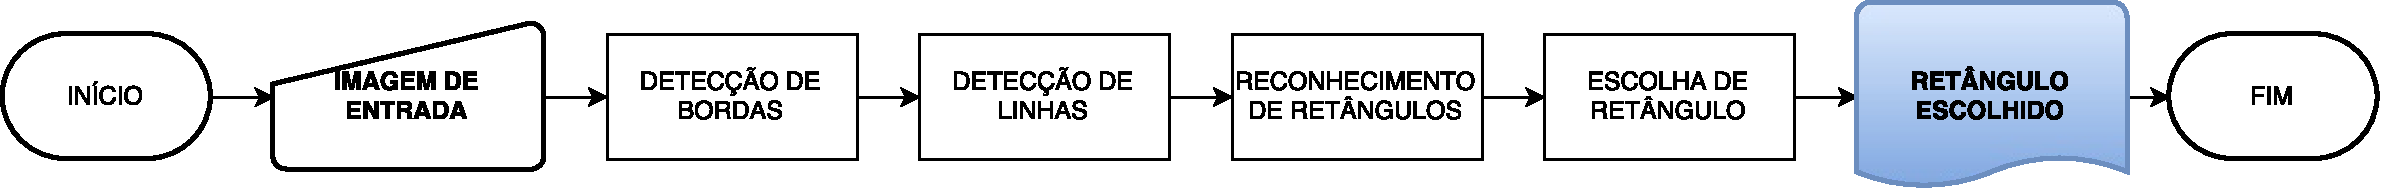
\includegraphics[width = \textwidth]{figuras/diaginicial.pdf} \label{testefigura}
\caption{Fluxograma do método de extração de telas de TV e monitores.}
\end{figure}

\section{Abordagem da Metodologia} \label{met:abord}

A utilização da metodologia descrita neste capítulo se encontra nas linhas de montagem de TVs e monitores. Em conjunto com um sistema gerador de sinais para a TV e com o auxílio de um sistema computacional para diagnóstico, esta metodologia fornece a base para um sistema que inspeciona aspectos operacionais e falhas possíveis em uma TV ou monitor, sem a necessidade de constante intervenção humana e com aumento da confiabilidade e rapidez, se comparado com a inspeção manual \cite{vantagemauto}. \textcolor{red}{MENCIONAR COMO VANTAGEM?: devido à metodologia, o sistema precisa de pouca ou nenhuma reprogramação, para o caso de diferentes modelos/tamanhos de tv, se for respeitada a proporção 16:9}

O modelo MRF apresenta uma alternativa para a detecção de retângulos robusta a diferentes tamanhos, orientações e cores de retângulo. Assim, a posição, cor ou orientação da TV ou monitor testados, assim como do fundo do ambiente onde a imagem é capturada, têm menor influência sobre o resultado da inspeção que nos sistemas propostos por outros trabalhos com tema semelhante \cite{inspect,vantagemauto}.

A análise de gradiente multi-dimensional é uma técnica para detecção de bordas em imagens coloridas robusta a mudanças na iluminação e cores da imagem. Isto apresenta uma vantagem sobre outras técnicas estudadas na literatura, que detectam bordas somente em imagens em escala de cinza \cite{canny,citasobel,roberts}. Isto se dá porque a informação de cor adiciona a tarefas de processamento de imagens, como segmentação e classificação, meios de aumentar tanto a eficácia quanto a variedade de aplicações \cite{bordacolor}.

\section{Detecção de Bordas} \label{met:borda}

%lembrar sempre que precisa haver a DESCRIÇÃO das técnicas utilizadas, assim como sua MOTIVAÇÃO (porque usei A e não B, que autores concordam cmg)
%\textcolor{red}{felipe, evite frases obvias... eh claro que eh importante.. outra coisa: comece indicando rapidamente o que ela e depois elabore...}

A detecção de bordas é a etapa inicial do método. Ela tem como entrada a imagem de entrada e dá como saída uma matriz binária chamada mapa de bordas, em que cada pixel que corresponde a uma borda na imagem tem valor 1 na matriz e os restantes têm valor 0. A teoria relacionada à detecção de bordas é abordada em detalhes no Capítulo \ref{refteor}. A Figura \ref{exemploborda} mostra um exemplo de extração de bordas de uma imagem.

%A borda de uma imagem é uma mudança significativa nos valores de intensidade de uma imagem, normalmente indicando uma mudança de região nela. Um mapa de borda da imagem é, portanto, uma matriz do mesmo tamanho da imagem, com pontos indicando a localização das bordas. A detecção de bordas é a área de processamento de imagem que estuda meios de localizar estas bordas \cite{borda01}. A Figura \ref{exemploborda} mostra um exemplo de detecção de bordas.

%Jain, R., Kasturi, R., & Schunck, B. G. (1995). Machine vision (Vol. 5). New York: McGraw-Hill.


\begin{figure}[h]
  \centering
  \subfloat[original]{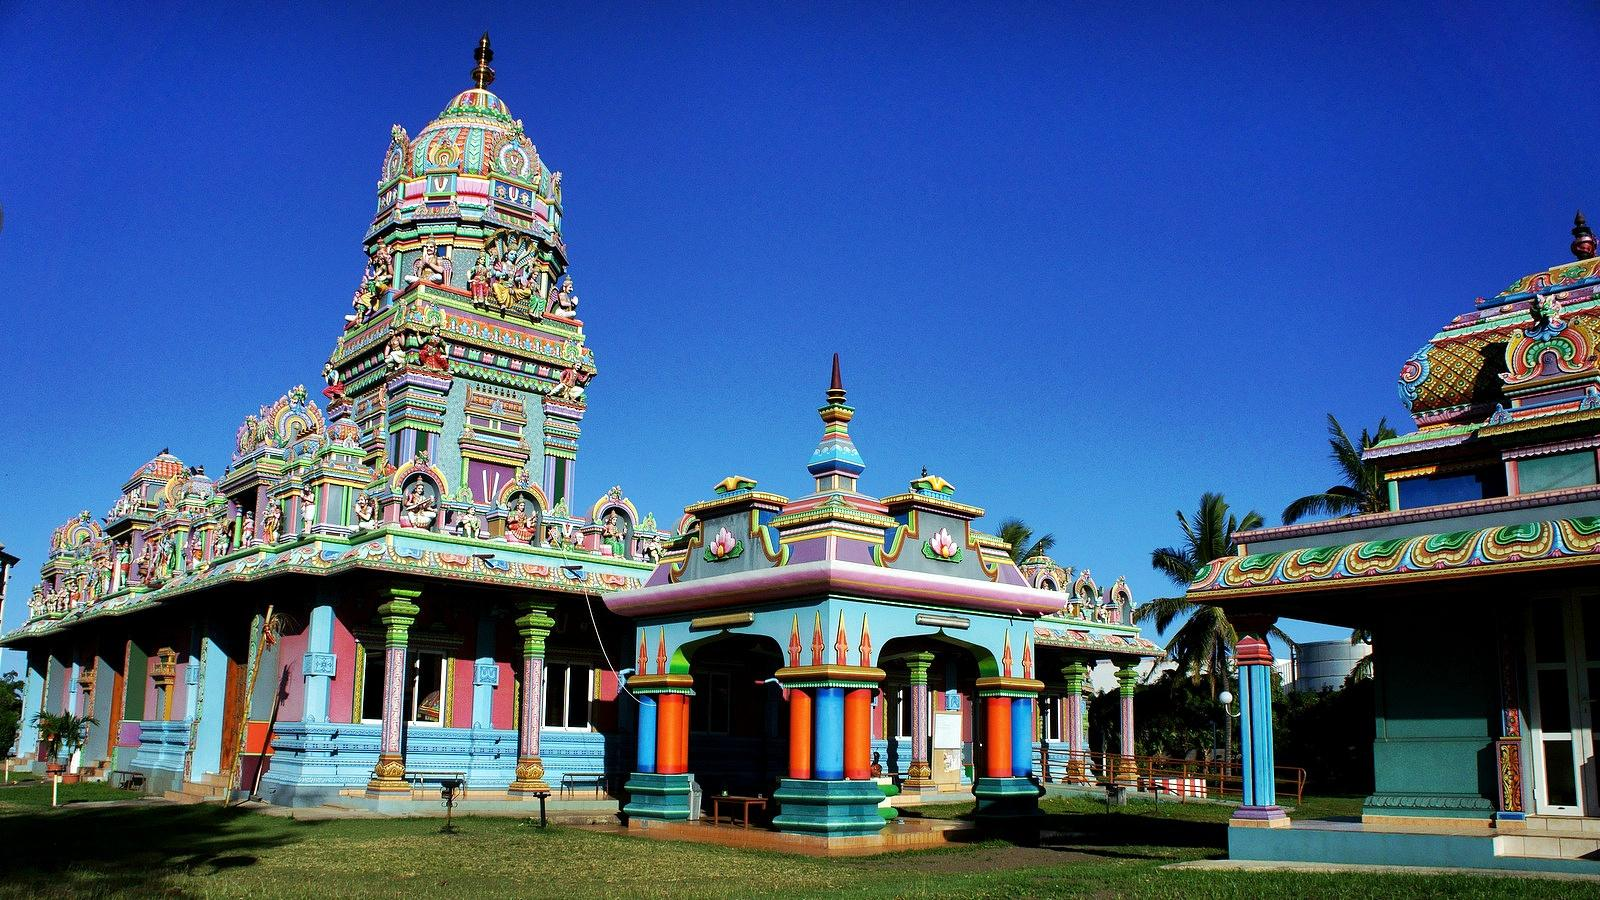
\includegraphics[width=0.45\textwidth]{figuras/fig1orig.jpg}\label{fig:f1}}
  \hfill
  \subfloat[borda]{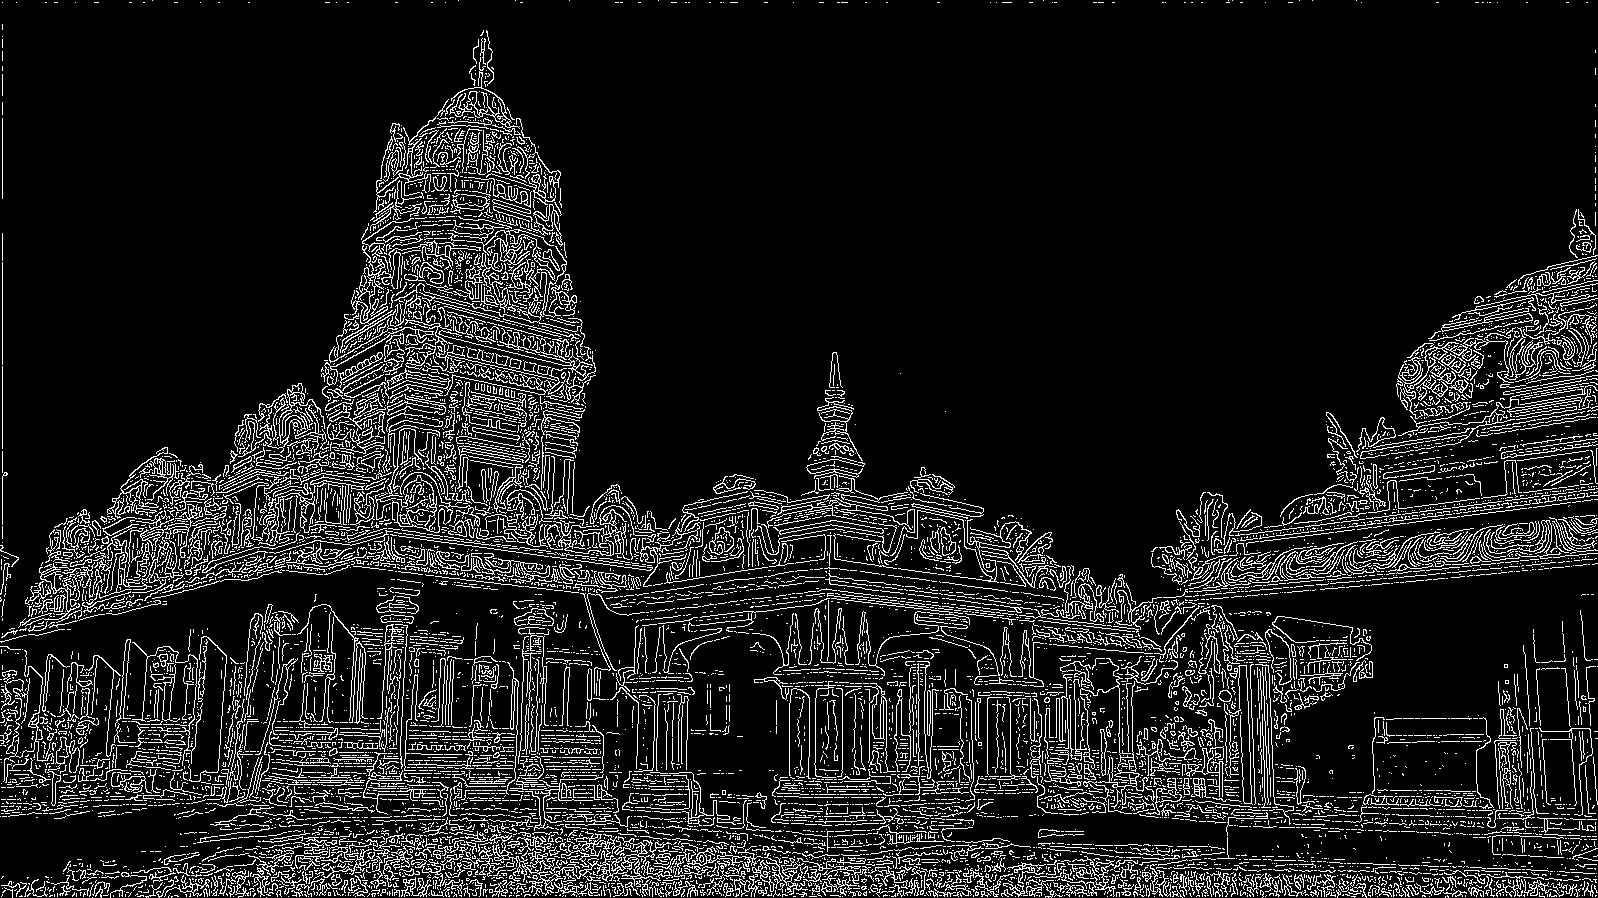
\includegraphics[width=0.45\textwidth]{figuras/fig1borda.jpg}\label{fig:f2}}
  \caption{Imagem e seu mapa de bordas.}
  \label{exemploborda}
\end{figure}


%A detecção de bordas é uma etapa de preprocessameto importante.
%Neste trabalho, a detecção de bordas é feita usando análise de gradiente multi-dimensional \cite{borda00}. Esta técnica considera a imagem um campo vetorial, ou seja, uma função no espaço $x,y$. Ela calcula seu gradiente para eleger candidatos a pixels de borda. Após isso, é implementando um esquema de seleção e verificação de candidatos para formar a imagem de borda. O pixel é selecionado como candidato caso sua magnitude de gradiente seja um máximo local. A verificação descarta candidatos caso o candidato não tenha vizinhos também candidatos e se a magnitude do gradiente daquele pixel for muito diferente da magnitude dos seus vizinhos na direção do gradiente.
%Através deste esquema, é possível detectar a borda de imagens coloridas no espaço RGB. Ele será mais detalhado a seguir.

%falar sobre como funciona o fluxo do processo. qual a utilidade de calcular o ggradiente, depois pra que fazer a seleção de candidatos e por último como e porque fazer a verificação. 

O esquema de detecção de bordas utilizado nesta dissertação é baseado na análise de gradiente multi-dimensional \cite{borda00} e no detector de Canny \cite{canny}. A imagem é tratada como um campo vetorial e são calculadas a magnitude e direção de seu 	gradiente. Utilizando esse esquema é possível obter o gradiente de imagens coloridas sem precisar recorrer à conversão para tons de cinza. A magnitude e direção do gradiente são informações úteis para a seleção de candidatos a pixeis de borda. Esta seleção é feita para separar, dentre os pixeis, os mais propícios a pertencerem a bordas de objetos com pouco custo computacional. A verificação, mais custosa computacionalmente que a seleção, é feita para descartar, dentre os pixeis anotados como candidatos, os que realmente não pertençam a uma borda.

As etapas do esquema de detecção de bordas serão detalhadas a seguir.

%Esta técnica é útil por funcionar bem em imagens coloridas e também por gerar informação de ângulo de gradiente, que vai ser útil nas próximas etapas do processamento.

%\textcolor{red}{aqui muita coisa tah faltando... mostre as formulas dos gradintes, coloque uma imagem ilustrando a selecao de candidatos e fale todos os detalhes que voce puder... nao economize palavras...}

%Illingworth, J., \& Kittler, J. (1988). A survey of the Hough transform.Computer vision, graphics, and image processing, 44(1), 87-116.


\subsection{Obtenção do Gradiente}

%\textcolor{red}{voce novamente comeca seco... fale o que isso eh...}

Um campo vetorial é uma construção matemática que aponta um vetor ou conjunto de vetores a cada valor de um espaço n-dimensional. Ele pode ser representado como:

$$ \textbf{f}:X \rightarrow \mathbb{R}^m $$

Em que $X$ é um subconjunto de $\mathbb{R}^m$ e $\textbf{f}$ pode ser composto por um ou mais vetores. Uma imagem pode ser considerada um campo vetorial cujo domínio é o espaço bidimensional e cujo contradomínio é composto por três vetores, um para cada elemento no espaço $RGB$, como mostrado em Lee e Cok \cite{borda00}.

Portanto, dado um campo vetorial representado pela função $ f: S \to \mathbb{R}^2 $, uma imagem no espaço $RGB$ pode ser representada como um subespaço de $f$ representado como $ V_{2 \to 3} $.

%Esta técnica considera uma imagem colorida como um campo vetorial que mapeia um espaço n-dimensional (espaço) em um m-dimensional (canais), como mostrado em [Lee e Cok] \textcolor{red}{nao referencie diretamente a referencia... coloque o nome dos autores e depois a ref... ex: como mostrado por Farias et al. [2]}. Portanto, dado um campo vetorial representado pela função $ f: S->R^m $, uma imagem pode ser representada como um subespaço de $f$ dado por $ Vn->m $.

%exemplos do professor: pode ser usado em outros tipos de representação de imagem?


%Dada uma imagem colorida, o gradiente é obtido calculando e depois combinando as seis derivadas de primeira ordem (duas pra cada canal R,G e B da imagem) e depois implementando um esquema de seleção e verificação de candidatos para formar a imagem de borda. Este esquema é composto por duas fases: um pixel é selecionado como candidato caso sua magnitude de gradiente seja maior que a magnitude dos seus vizinhos na direção do gradiente. A fim de evitar ruído, a verificação descarta candidatos segundo dois critérios: se o candidato não tem vizinhos também candidatos, e se a magnitude do gradiente daquele pixel é muito diferente da magnitude dos seus vizinhos na direção do gradiente.

A derivada da função $f$ nestas condições pode ser representada pela matriz $D$ tal que:

$$ f' = D = \begin{bmatrix} 
\frac{\partial r}{\partial x} & \frac{\partial r}{\partial y} \\
\frac{\partial g}{\partial x} & \frac{\partial g}{\partial y} \\
\frac{\partial b}{\partial x} & \frac{\partial b}{\partial y} \\ 
\end{bmatrix} $$

Saindo de um ponto $x$ qualquer na imagem, o deslocamento $d$ na direção do vetor unitário $\textbf{u}$ é dado pela equação:

$$d = \sqrt[]{\textbf{u}^TD^TD\textbf{u}}$$

O maior valor de $d$, ou seja, o gradiente deste vetor, é dado pelo maior autovalor de $D^TD$. Definindo as variáveis $Mxx$, $Mxy$ e $Myy$ como:
%Considerando uma imagem bidimensional com três canais (um para cada canal de cor r, g e b), $DV$ é a matriz que mostra a variação dos valores de R, G e B no espaço infinitesimal dx e dy. 

%$$ DV = (dx dy)Jc^T $$ 

%\textcolor{red}{para alinhar a esquerda, use 'noindent'...}

%em que $Jc$ é a matriz jacobiana, que tem a seguinte forma:

%$$ Jc = \begin{bmatrix} 
%\frac{\partial r}{\partial x} & \frac{\partial r}{\partial y} \\
%\frac{\partial g}{\partial x} & \frac{\partial g}{\partial y} \\
%\frac{\partial b}{\partial x} & \frac{\partial b}{\partial y} \\ 
%\end{bmatrix} $$

%$ DV^2 $ é a matriz que mostra a taxa de variação dos valores da matriz $DV$. Ela é dada por:

%$$ DV^2 = (dx dy)Mc(dx dy)^T $$

$$ Mxx = (\frac{\partial r}{\partial x})^2+(\frac{\partial g}{\partial x})^2+(\frac{\partial b}{\partial x})^2 $$

$$ Mxy =(\frac{\partial r}{\partial x})(\frac{\partial r}{\partial y})+(\frac{\partial g}{\partial x})(\frac{\partial g}{\partial y})+(\frac{\partial b}{\partial x})(\frac{\partial b}{\partial y}) $$

$$ Myy = (\frac{\partial r}{\partial y})^2+(\frac{\partial g}{\partial y})^2+(\frac{\partial b}{\partial y})^2 $$

podemos definir $D^TD$ como:

$$ D^T D = \begin{bmatrix} Mxx & Mxy \\ Mxy & Myy \end{bmatrix}$$


O maior autovalor de $D^TD$ é dado por:

$$ V = (\sqrt{( (Mxx+Myy)^2 - 4 x(Mxx \times Myy - (Mxy)^2 ) )}+Mxx+ Myy)/2 $$

e seu autovetor correspondente é $ \{Mxy,V-Myy\}/2 $. Portanto a direção do gradiente é dada por:

$$ \theta = tan^{-1}((V-Mxx)/Mxy) $$

A raiz quadrada do maior autovalor $V$ e seu autovetor correspondente são equivalentes à magnitude e direção do gradiente em um ponto da imagem. Portanto, para cada pixel $(i,j)$, seu gradiente é encontrado computando seus autovalores e autovetores com as equações acima descritas.

%\textcolor{red}{aqui valem o mesmos comentarios da secao anterior e ainda tem o fato de voce ter colocado exatamente como estah no artigo dos caras... nao faca isso... o leitor tem que ver que voce colocou o seu entendimento e nao uma copia do que leu... Por exemplo, comente sobre o significado da jacobiana, fale se isso pode ser usado em outras imagem com tres canais (HSV, Lab, etc...) e gaste bastante texto explicando cada um dos elementos: V, Mxy, Myy e $\theta$... manjou?}


\subsection{Detecção de Candidatos}

%\textcolor{red}{nao dah para deixar uma secao com este tamanho... fale mais e coloque uma figura... os mesmos comentarios da primeira secao valem aqui}

A detecção de candidatos a pixel de borda é o primeiro passo para obtenção da imagem de borda. Ela filtra a imagem em busca de candidatos que serão depois selecionados em um sistema de verificação, mais custoso computacionalmente.

Primeiramente é calculada a matriz $D^TD$, assim como seus valores de $V$ e $\theta$, para cada um dos pixels da imagem. A detecção de candidatos a pixel de borda é feita analisando esta informação. São considerados candidatos os pixeis cuja magnitude é uma máxima local, ou seja, os pixeis cuja magnitude seja maior que a dos seus dois vizinhos na direção do gradiente, são considerados candidatos a pixeis de borda. Isto pode ser melhor exemplificado pela Figura \ref{maxlocal}.

%Após calcular a matriz $Mc$ para cada pixel da imagem e seus valores de $V$ e $\theta$, os pixeis com máxima local de magnitude de gradiente na direção dele, ou seja, os pixeis cuja magnitude seja maior que a dos seus dois vizinhos na direção do gradiente, são considerados candidatos a pixeis de borda.

\begin{figure} [h]
\centering
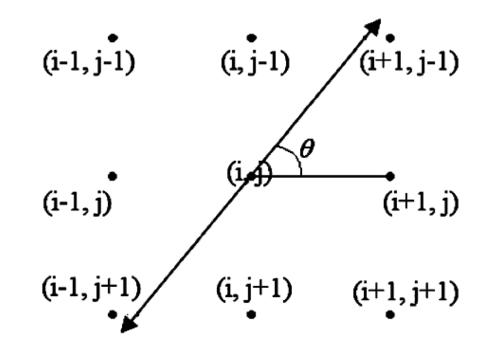
\includegraphics[width = 0.5\textwidth]{figuras/vizinh.jpg} \label{maxlocal}
\caption{Direção de gradiente de um pixel e seus vizinhos. Adaptado de \cite{mrf}.}
\end{figure}

\subsection{Verificação de Candidatos}

A verificação é um processo necessário para descartar os pixeis cujo gradiente é uma máxima local mas não são pixeis de borda. Isto pode ocorrer devido a ruído (adquirido na aquisição da imagem, devido à curvatura da lente ou à quantização), diferenças na iluminação dos objetos, efeitos de luz e sombra ou oclusão de objetos \cite{ruidocausas}.

%, como os gerados por ruído \textcolor{red}{coloque uma refe aqui... que tipo de ruido? de onde?}. 

Esta verificação é baseada em operações que se aproveitam das informações obtidas anteriormente e de análise das regiões das imagens. Elas são livremente baseadas na etapa de verificação de candidatos do detector de bordas de Canny \cite{canny}:

%\textcolor{red}{novamente voce economiza palavras... assim nao da... coloque tudo... quero figuras, explicacoes, insights, modificacoes, etc.}

\begin{itemize}
\item Primeiramente, a vizinhança do pixel é analisada. O candidato a pixel de borda deve ter vizinhos também candidatos. Se nenhum dos oito pixeis vizinhos for um candidato a pixel de borda, aquele pixel é considerado ruído e descartado;
\item Foi percebido que não há variação muito grande entre as magnitudes de pixeis de borda vizinhos \cite{mrf}. Portanto, é calculada a diferença entre magnitude do gradiente dos pixeis vizinhos. Caso esta diferença seja grande demais, o pixel é descartado. A seguinte inequação é definida para avaliar a diferença:
\begin{equation}
(sum(| V(i,j) - V(i+p,j+q) |)- sum(V(i+p,j+q))) >0
\end{equation}


\end {itemize}

\section{Detecção de Linhas} \label{met:linha}

%\textcolor{red}{nao vou nem comentar isso... ajeite...}

%Após detectar as bordas da imagem, se faz necessário ligar os pixeis de borda vizinhos e com orientações semelhantes em conjuntos de segmentos de retas. Com isso, é preparado o terreno para a próxima etapa, que rotula linhas como pertencentes a objetos retangulares. 

%A identificação de linhas é feita utilizando a transformada de Hough. Devido ao ruído e a diferenças na iluminação, é possível que segmentos de reta tenham descontinuidades. Para atacar este problema, é implementado um esquema para mesclar segmentos que pareçam pertencer à mesma linha (\textbf{manter o texto desse jeito? não ta muito informal?}) \textcolor{red}{tah bem ruim...}

Esta seção apresenta o esquema de identificação de linhas em uma imagem deste método. A identificação é baseada na transformada de Hough \cite{houghintro00}, uma técnica que facilita o trabalho de encontrar linhas e outros padrões complexos em imagens binárias ao transformar estes padrões em conjuntos de parâmetros mais facilmente identificáveis. Sua aplicação para encontrar linhas é baseada na parametrização popularizada por Duda e Hart em \cite{houghintro02}.

Os segmentos encontrados na transformada não necessariamente correspondem às linhas dos objetos que as fotos representam. Descontinuidades em retas podem aparecer devido a diferenças na iluminação ou reflexos. Portanto, as linhas encontradas pela transformada são posteriormente submetidas a um esquema de  mesclagem e seleção, de forma que somente os segmentos relevantes para o reconhecimento de retângulos seja dada como resultado final. A mesclagem é feita analisando as propriedades espaciais das linhas encontradas, juntando as que têm orientação e distância da origem semelhantes e eliminando as que têm ângulo muito diferente de 90º e 0º.

\subsection{Transformada de Hough}

%\textcolor{red}{cade o texto falando rapidamente sobre a transformada? como ela surgiu? qual era o objetivo? encontrar pontos com mesmo rho e theta, o que significa que provavelmente fazem parte da mesma linha... e a votacao? cade as figuras? que variante de hough foi usada?... os mesmos comentarios das secoes anteriores valem aqui... e para de fazer tudo a prestacao... coloque as imagens logo...}

A transformada de Hough foi criada por P.V.C Hough para detectar padrões complexos em imagens binárias. Para atingir este objetivo, são determinados parâmetros que caracterizam estes padrões. Assim, o problema de detectar um padrão em uma imagem binária é transformado no problema de detectar um valor no espaço paramétrico \cite{houghintro01}.

%fonte: VC, H. P. (1962). U.S. Patent No. 3,069,654. Washington, DC: U.S. Patent and Trademark Office.

No caso específico de detecção de retas, a transformada de Hough funciona transformando uma linha reta em um ponto no espaço paramétrico. Os parâmetros utilizados por Hough para caracterizar uma reta no espaço $x,y$ são a inclinação $m$ e interseção $b$, portanto a reta $y = mx+b$ é representada como um ponto no espaço $m,p$.

Supondo que se tenha um conjunto de $n$ pontos em uma imagem $N = \{(x_1,y_1),(x_2,y_2),...,(x_n,y_n)\}$  e se queira descobrir a que linha eles pertencem, são computadas todas as retas que passam por aquele conjunto de pontos. Para cada reta que contém um dos pontos é computado um voto no espaço paramétrico $m,b$. Assim, a reta com maior número de votos é considerada a reta a qual os pontos pertencem. Este processo pode ser melhor representado na Figura \ref{houghpuro}

\begin{figure}[h]
  \centering
  \subfloat[imagem original]{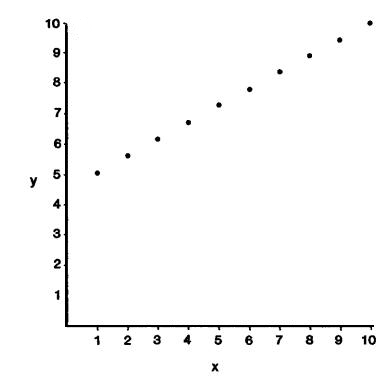
\includegraphics[width=0.4\textwidth]{figuras/houghpuro00.jpg}\label{houghpuro:f1}}
  \hfill
  \subfloat[representação no espaço paramétrico]{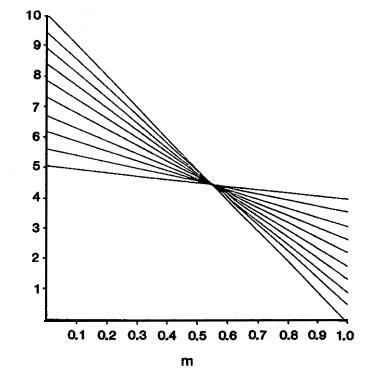
\includegraphics[width=0.4\textwidth]{figuras/houghpuro01.jpg}\label{houghpuro:f2}}
  \caption{imagem com pontos colineares e sua representação no espaço $m,b$. Adaptado de \cite{houghintro01}.}
  \label{houghpuro}
\end{figure}

Entretanto, a parametrização no espaço $m,b$ não consegue representar corretamente linhas verticais ou próximas desta inclinação, como perceberam Duda e Hart em seu influente artigo \cite{houghintro02}. A fim de eliminar estes problemas, eles propuseram uma nova parametrização para a transformada de Hough. Nela, as retas no espaço $x,y$ são representadas no espaço $\rho,\theta$, onde $\rho$ é a distância entre a origem da imagem e a reta, pelo seu ponto mais próximo, e $\theta$ é o ângulo que a normal à reta faz com o eixo $x$. A equação da reta, portanto, é dada por: 

$$\rho = x cos \theta +y sin \theta $$ 

%fonte: Duda, R. O., & Hart, P. E. (1972). Use of the Hough transformation to detect lines and curves in pictures. Communications of the ACM, 15(1), 11-15.

%FIGURA COM UMA RETA MOSTRANDO RHO E THETA

\begin{figure} [h]
\centering
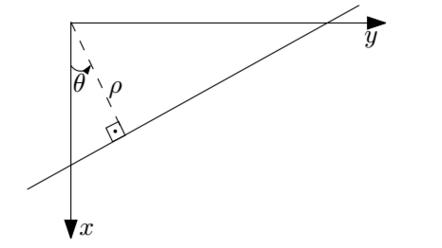
\includegraphics[width = 0.6\textwidth]{figuras/hough.jpg} \label{hough} \caption{Representação paramétrica de Hough. Adaptado de \cite{hough00}}
\end{figure} 

%imagem de: Jung, C. R., & Schramm, R. (2004, October). Rectangle detection based on a windowed Hough transform. In Computer Graphics and Image Processing, 2004. Proceedings. 17th Brazilian Symposium on (pp. 113-120). IEEE.

Assim, dado um pixel de borda, para cada possível reta que passe por ele, é computado um ponto no espaço $(\rho,\theta)$. O conjunto de linhas possíveis passando por um determinado ponto forma um sinusoide naquele espaço. Com dois ou mais pontos na imagem pertencendo à mesma linha, as sinusoides que os representam se tocam justamente no ponto que representa a mesma. Isto é melhor representado na imagem \ref{houghlinhas}, que mostra uma imagem com dois pontos brancos e sua representação no espaço de Hough.

%FIGURA REPRESENTANDO DOIS PONTOS LIGADOS À MESMA LINHA E O SEU ESPAÇO PARAMÉTRICO

\begin{figure}[h]
  \centering
  \subfloat[imagem original]{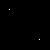
\includegraphics[width=0.35\textwidth]{figuras/houghpts0000.jpg}\label{houghlinhas:f1}}
  \hfill
  \subfloat[representação no espaço de Hough]{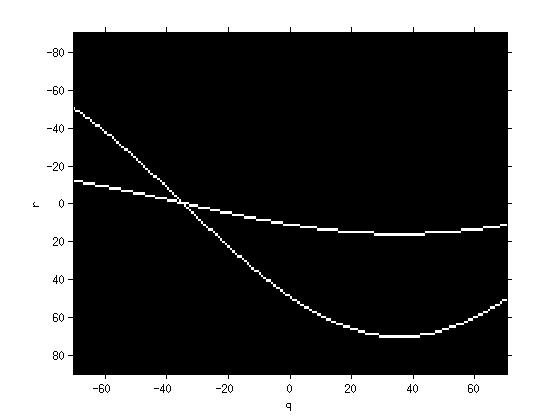
\includegraphics[width=0.5\textwidth]{figuras/houghpts0001.jpg}\label{houghlinhas:f2}}
  \caption{imagem com dois pontos e a representação paramétrica.}
  \label{houghlinhas}
\end{figure}


O algoritmo para encontrar linhas utilizando a transformada de Hough, portanto, tem os seguintes passos: 
\begin{itemize}
\item escanear toda a imagem de borda e computar, para cada pixel assinalado como borda, seu conjunto de coordenadas no espaço paramétrico $(\rho,\theta)$. Os parâmetros rho e theta são quantizados com um $d\rho = 10$ e $d\theta = 1$;
\item escanear o espaço paramétrico e encontrar os pontos que mais se interceptam. A fim de evitar linhas pequenas demais, é estabelecido um limiar mínimo de tamanho das linhas;
\item para cada um dos pontos assinalados no espaço paramétrico, procurar os pontos da imagem que passam por aquela reta para assinalar iniciais e finais das linhas;
\end{itemize}

\subsection{Esquema de Mesclagem de Linhas}

Utilizando os conhecimentos sobre o problema e análise espacial das linhas, foram desenvolvidos esquemas para mesclar segmentos de reta que foram separados por culpa do ruído ou de diferenças na iluminação, assim como para eliminar linhas que têm pouco valor para as próximas etapas do processamento.

%mesclar linhas próximas

Iluminação ou ruído podem interferir na correta detecção de linhas. Com isso, o mesmo segmento pode acabar sendo detectado como dois segmentos menores. A fim de atacar este problema, esta parte do algoritmo mescla linhas encontradas no processo anterior segundo os seguintes critérios:
\begin{itemize}
\item As linhas devem ter orientação e distância da origem semelhante. Devido ao ruído e a problemas na quantização, é possível que algumas linhas do mesmo segmento tenham orientação ou distância da origem um pouco diferentes entre si;
\item A distância entre os segmentos deve ser muito pequena (não maior que 5 pixeis);
\item Segmentos paralelos não podem se sobrepor significativamente quando projetados na direção perpendicular à linha;
\end{itemize}


%eliminar linhas com ângulos muito diferentes de 90º e 0º

Aproveitando-se das características geométricas particulares de telas de TV e monitores, esta parte do algoritmo busca descartar linhas que têm ângulos muito diferentes de 0º e 90º. Assim, não só a próxima etapa terá menos linhas para analisar quanto eliminará linhas que podem gerar falsos positivos.
Ele faz uma busca em todas as linhas encontradas, selecionando as que têm ângulo fora da faixa entre 0º e 5º e 85º e 90º e eliminando-as da lista de linhas a se analisar.

Através deste esquema, são identificados e selecionados os segmentos de reta pertencentes à imagem de borda que serão utilizadas na detecção de retângulos.

%fonte: 

%Duda, R. O., & Hart, P. E. (1972). Use of the Hough transformation to detect lines and curves in pictures. Communications of the ACM, 15(1), 11-15.

%Illingworth, J., & Kittler, J. (1988). A survey of the Hough transform.Computer vision, graphics, and image processing, 44(1), 87-116.


\section{Reconhecimento de Retângulos} \label{met:retangulo}

%problema
Após identificar as linhas presentes na imagem e eliminar as que não são interessantes, é necessário classificar as linhas encontradas como pertencentes ou não ao lado de um objeto retangular. Neste trabalho, a classificação é feita através de um modelo baseado no Campo Aleatório de Markov (MRF). A teoria do MRF utiliza as relações entre elementos vizinhos para estimar o estado futuro de seus elementos. Portanto, é criado algoritmo baseado neste modelo para rotular as linhas encontradas.
%Um Campo Aleatório de Markov pode ser utilizado para modelar entidades tais como pixels ou linhas, caracterizando as relações entre as entidades utilizando as distribuições

%Para classificar linhas como parte de um retângulo é necessário um modelo que leve em conta as relações entre elas. O Campo Aleatório de Markov é uma ferramenta que utiliza justamente as relações entre elementos vizinhos para estimar o estado futuro de seus elementos. Portanto, é criado algoritmo baseado neste modelo para rotular as linhas encontradas.
%como funciona mrf
%\textcolor{red}{nao da para falar de cadeias de markov sem referencias... isso vale para todo o texto... onde tiver uma afirmacao ou algo que nao foi explicado diretamente no texto, coloque uma referencia}

%\textcolor{red}{vou parar aqui... tudo que eu falei anteriormente vale para todo o texto...}

%Processo Estocástico definição

%Variável aleatória definição

Esta seção abordará os principais conceitos relativos ao MRF, a formação e necessidade do Sistema de Vizinhanças, o funcionamento do algoritmo de classificação e a posterior escolha do retângulo que representa a tela, assim como seu redimensionamento.

\subsection{Campo Aleatório de Markov (MRF)}

Um Campo Aleatório de Markov (MRF) é um processo estocástico que apresenta propriedade Markoviana. A definição desta propriedade, assim nomeada em homenagem a Andrei Markov, é que o estado futuro de um processo pode ser previsto sabendo apenas o estado atual, ignorando seus estados anteriores.

\subsubsection{Conceitos Iniciais}

A teoria relativa ao MRF utiliza diversos conceitos da estatística que podem não ser familiares. A fim de melhor entendimento da seção, alguns deles serão expostos abaixo: 

\begin{itemize}

\item \textbf{variável aleatória} é o nome dado a uma variável cujo valor não é exato, mas sim pode ter uma série de valores, cada um deles associado a uma probabilidade. Neste trabalho, variáveis aleatórias serão representadas por uma letra latina maiúscula:

$$ X $$

E sua probabilidade de apresentar valor $x$ será representada como segue:

$$ P(X = x)$$

\item \textbf{Processo estocástico}, ou processo aleatório, é um conjunto de variáveis aleatórias que representam a evolução de um mesmo sistema ao longo do tempo. Dado um conjunto de variáveis aleatórias $X$ e o tempo $T$ formado pelos passos $t$, um processo estocástico pode ser representado por:

$$ \{X_t,t\subset T\}$$

Em que $X_t$ representa o estado do processo no tempo $t$.

\item \textbf{Campo aleatório} é um conjunto de variáveis aleatórias. A diferença para o processo estocástico é que o parâmetro que une estas variáveis não precisa ser necessariamente o tempo. O MRF é um tipo de campo aleatório.

\end{itemize}

A teoria do MRF permite modelar a probabilidade \textit{a priori} de elementos relacionados entre si. Em conjunto com teorias de estimação, é formulada uma função objetiva para estimar os valores das variáveis aleatórias. Esta função pode ser encaixada em um algoritmo devido a um teorema que equivale o MRF a uma distribuição de Gibbs.

Para caracterizar as relações entre os elementos pertencentes ao MRF é criado um sistema de vizinhanças. Este sistema utiliza as informações espaciais das linhas para estabelecer as relações entre elas.

%As probabilidades/o estado futuro dos elementos do modelo MRF dependem das inter-reações entre eles e seus elementos vizinhos. Para caracterizar estes elementos, um sistema de vizinhança é criado.

%(1.1 da referencia)

%Portanto, dada a variável aleatória $X$, $X_n$ representa seu estado no passo $n$. Caso $X$ seja parte de uma Cadeia de Markov, a probabilidade de $X_{n+1}$ ser igual a um estado $x$ é dada por:

%$$ P(X_{n+1} = x|X_1,...,X_n ) = P(x|X_n) $$



%O MRF é uma técnica adequada para a resolução do problema porque a probabilidade de uma linha vir a pertencer ao lado de um retângulo depende principalmente dos seus vizinhos. Mapeando estas características, é possível montar um modelo MRF para rotular segmentos. Primeiramente, um sistema de vizinhanças é formado para prover o modelo de informações espaciais sobre as linhas. Após isto, um algoritmo de aprendizado utiliza estas informações para rotular as linhas como pertencentes a um lado de retângulo.

\subsubsection{Sistema de Vizinhanças}

Um campo aleatório é considerado um MRF se a probabilidade condicional de um elemento depender de seus elementos vizinhos \cite{vizinh00}. O sistema de vizinhanças caracteriza os elementos do campo como vizinhos ou não entre si.

%MELHORAR O sistema de vizinhanças foi criado para fornecer ao modelo MRF as informações relativas às linhas. Estas informações são obtidas explorando características espaciais das mesmas. Características estas que são

%fonte: Wang, X., & Wang, H. (2004). Evolutionary optimization with Markov random field prior. Evolutionary Computation, IEEE Transactions on, 8(6), 567-579.

O sistema de vizinhança é caracterizado como segue: o conjunto de elementos vizinhos do elemento $l_i$ é representado por $N(l_i)$. Pertencem a $N(l_i)$ elementos que observem as seguintes condições:
\begin{itemize}
\item $l_i$ não pertence a $N(l_i)$ 
\item se $l_j$ pertence a $N(l_i)$, $l_i$ pertence a $N(l_j)$.
\end{itemize}
No caso específico deste modelo, os elementos são linhas. A vizinhança é caracterizada utilizando suas relações espaciais. Para uma linha $lj$ ser considerada vizinha de $li$, ela deve obedecer a três condições:
	\begin{itemize}
\item $lj$ deve ser paralela ou perpendicular a $li$. Uma variável $H(i,j)$ é formada para avaliar as relações espaciais entre as linhas $li$ e $lj$. Se $H(i,j) = 1$, $li$ e $lj$ são perpendiculares entre si, ao passo que se $H(i,j) = 0$, $li$ e $lj$ são paralelas. Caso os ângulos entre $li$ e $lj$ não pertençam a nenhuma das categorias anteriores, $H(i,j) = -1$;
\item A distância $D(i,j)$ entre $li$ e $lj$ não pode ser muito grande ou muito pequena. A distância é computada de duas formas, dependendo de $H(i,j)$. Caso $H(i,j) = 0$, a distância entre $li$ e $lj$ é a menor distância entre as duas linhas, ou seja, o comprimento de uma reta normal às duas que toca as duas linhas. Neste caso, $D(i,j)$ deve ser menor que o Maior Tamanho de Retângulo possível (MRS), normalmente igual ao tamanho da imagem, e maior que o Menor Retângulo Possível (MIS).  Caso $H(i,j) = 1$, a distândia é considerada a menor distânca entre o dim de um segmento e outro segmento. Neste caso, $D(i,j)$ deve ser menor que metade do tamanho do menor segmento;
\item Por último, se $li$ e $lj$ são paralelos, eles devem se sobrepor em uma porção significativa quando projetados na direção prependicular às linhas. Se a sobreposição for superior a 60\% do tamanho das linhas, elas podem ser vizinhas. 
\end{itemize}
 A figura \ref{uelinha} ilustra as condições explicadas. Nela, $l1$ e $l2$ são linhas paralelas, $l3$ é uma linha perpendicular às duas, $D(1,2)$ é a distância entre $l1$ e $l2$ e $D(2,3)$ é a distância entre $l2$ e $l3$. A projeção da sobreposição da linha $l1$ na linha $l2$ é o segmento $AB$. Somente se $AB > 0.6*max(tam_l1,tam_l2)$, $l2$ será considerado vizinho de l1.

%FIGURA 2 DA REFERENCIA ZERO

\begin{figure} [h]
\centering
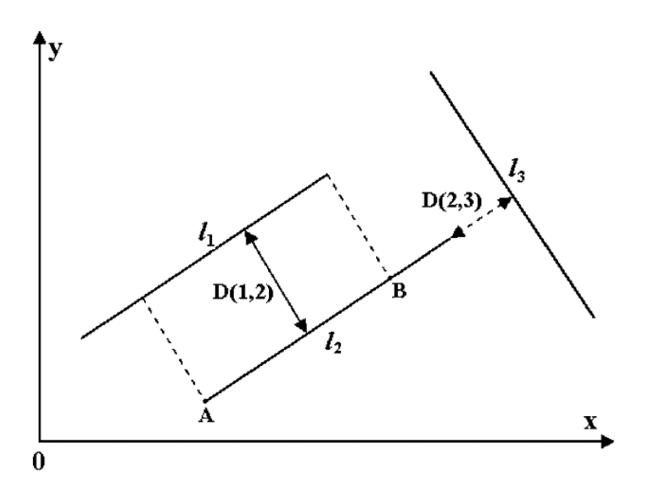
\includegraphics[width = 0.6\textwidth]{figuras/linhasparal.jpg} \label{uelinha} \caption{Linhas paralelas e perpendiculares. Adaptado de \cite{mrf}.}
\end{figure} 

%figura de: Liu, Y., Ikenaga, T., & Goto, S. (2007). An MRF model-based approach to the detection of rectangular shape objects in color images. Signal Processing, 87(11), 2649-2658.

%Com o sistema de vizinhanças descrito acima, o conjunto F é assumido como um MRF com suas características locais, para

%$$ i \in d, P(F_i|F_j,j \in d, j \neq i) = P(F_i|F_j, j \in N(l_i)) $$

\subsubsection{Algoritmo de classificação}

O problema de classificação encarado neste trabalho pode ser caracterizado a seguir. Seja $L = \{l_1,l_2,...,l_n\}$ o conjunto de segmentos de linha encontrados no processo anterior, $d = \{1,2,..,n\}$ o conjunto de indices de $L$ e $F = \{F_1,F_2,...,F_n\}$ uma família de variáveis aleatórias, em que cada variável $Fi$ toma um valor $f_i$ no espaço $[0,1]$. Este valor indica a probabilidade da linha $l_i$ pertencer ao lado de um objeto retangular.

O evento da variável $F_i$ ter o valor $f_i$ é representado como $F_i = f_i$. O evento conjunto em que o cada uma das variáveis de $F$ apresenta um conjunto de valores $ f = \{f_1,f_2,...,f_n\} $ é representado como $(F_1=f_1,...,F_n=f_n)$, ou $F = f$. O conjunto de valores $f$ é chamado de \textit{configuração} de $F$. A probabilidade deste evento conjunto é representada por $P(F=f)$

  %    b.   rotulando segmentos de linha

Sendo $F$ um MRF, a probabilidade de qualquer evento referente a ele depende de sua vizinhança. Essa vizinhança, encontrada na subseção anterior, é representada por $ N = \{N(l_i)| \forall i \in d\} $ e é a coleção de segmentos vizinhos a um segmento de linha $l_i$. 

Devido à equivalência entre o MRF e a distribuição de Gibbs \cite{mrfgibbs}, a probabilidade deste evento pode ser calculada seguindo esta distribuição, que é como segue:

\begin{equation} \label{eqgibbs}
 P(F = f|L) = Z^{-1} exp[\frac{-E(f)}{T}] 
\end{equation}

Em que $T$ é a temperatura, $Z$ é o fator de normalização e $E(f)$ é a função de energia posterior $ E(f)=U(f)/T+U(l|f) $, onde $U(f)$ e $U(l|f)$ são respectivamente a energia anterior e a energia de aproximação.

%$ P(F=f|L) $ é a distribuição posterior do MRF.

A maior parte dos problemas de visão computacional e processamento de imagens é tratada como um problema de otimização\cite{li2009markov}. Isto se deve ao alto grau de incertezas que permeia qualquer processo que envolva imagens. Ruído, descontinuidades e oclusão de parte dos objetos são geradores de incertezas, portanto é muito difícil obter uma solução exata. Uma solução inexata, porém ótima, é mais facilmente obtida.

A função de energia tem um papel importante nestes tipos de problema. Ela pode ser usada como uma medida da qualidade da solução, assim como facilita a procura por uma solução mínima, ou ótima. Uma função de energia bem projetada tem seu valor mínimo quando a solução é ótima.

Assim, o reconhecimento de lado do retângulo pode ser encarado como o seguinte problema: para um dado $L$, $ arg max \quad  P(f_i|l_i) $ para cada $ l_i $ é encontrado por $arg min \quad E(f) $, ou seja, minimizar a função de energia vai maximzar a probabilidade definida na equação \ref{eqgibbs}.

Maximizar esta probabilidade vai dar a máxima estimativa posterior de potenciais lados de retângulos na imagem de bordas. A função de energia $ E(f) $ é minimizada enquanto cada $ f_i $ é convergido para 0 ou 1. A função $ E $ consiste nos quatro termos a seguir:

\begin{equation}
E_1 = \alpha _1 {\sum_{i=1}^{n} {\sum_ {j\in N(l_i)}^{}f_if_jD(i,j)}} \label{e1}
\end{equation}

\begin{equation}
E_2 = \alpha _2 {\sum_{i=1}^{n} (\frac{f_i}{LEN_i}\times AVGLEN)}  \label{e2}
\end{equation}

\begin{equation}
E_3 = -\alpha _3 {\sum_{i=1}^{n} (f_i \ln f_i + (1-f_i)\ln(1-f_i))} \label{e3}
\end{equation}

\begin{align}
E_4 = \alpha_4 \sum_{i=1}^{n} \sum_ {j\in N(l_i)}^{}f_if_j \{ H(i,j)\times \min_{k\in (N(l_i)\cap N(l_j))} \frac{D(k,i)+D(k,j)}{f_k} +\\ \nonumber
(1-H(i,j))\times \min_{k\in (N(l_i)\cap N(l_j))} \frac{D(k,i)+D(k,j)}{f_kH(k,j)} \}
\label{e4}
\end{align}

Onde $ \alpha _1 $, $ \alpha _2 $, $ \alpha _3 $ e $ \alpha _4 $ são constantes positivas que controlam as contribuições de cada termo individual da função de energia. AVGLEN é o comprimento médio do conjunto de segmentos L:
	
$$ AVGLEN = \frac{1}{n} \displaystyle \sum_{i=1}^{n} LEN_i $$

$E_1$ apoia o agrupamento de segmentos próximos uns dos outros. $E_2$ favorece segmentos longos. $E_3$ é a entropia da configuração ${f_i}$, empurrando os ${f_i}$ para 0 ou 1. Por fim, $E_4$ favorece dois segmentos vizinhos, ambos próximos de um dos seus vizinhos em comum.

Os $ {f_i} $ são todos inicializados em 0.5 e a energia é gradualmente reduzida usando um algoritmo gradiente descendente com uma esquema de aprendizado.

$$ {f_i}_{(t+1)} = {f_i}_t - \mu_t \nabla E $$

$$ \mu_{(t+1)} = \mu_t - \beta $$

em que $\mu$ é um parâmetro de passo positivo, que influencia na taxa de convergência, $\beta$ é um pequena constante que faz o tamanho do passo diminuir a cada iteração, e $ \nabla E $ é o gradiente de $E$.

Minimizando a energia, os segmentos de $L$ cujo $f_i \simeq 1$ são selecionados como lados de objetos retangulares desconhecidos. Se faz necessário, então, um sistema que utilize as informações espaciais das linhas escolhidas para agrupar as linhas selecionadas em seus respectivos retângulos.

O sistema de vizinhanças foi construído para prover estas informações espaciais. Após rotulados os segmentos de linha, é feita uma busca em seus segmentos vizinhos a fim de formar retângulos integrados. Dado um segmento de linha $l$, marcado como pertencente a um retângulo, serão selecionados outros três segmentos também marcados da sua vizinhança, um dos quais será paralelo e os outros dois perpendiculares à linha, para formar um retângulo. Como última confirmação, os três segmentos devem ser vizinhos uns dos outros.

Com o esquema acima descrito, é possível reconhecer objetos retangulares em imagens coloridas agrupando segmentos de linha de quatro em quatro.

\subsection {Escolha do Retângulo que Representa a Tela}

A escolha do retângulo que representa a tela do monitor utiliza critérios criados através da análise das propriedades geométricas de uma tela de TV e de características da captura das imagens. O retângulo é escolhido como tela de TV caso:

\begin{itemize}
\item não esteja nas bordas da imagem
\item  tenha uma razão de aspecto próxima da dos monitores
\item tenha formato retangular
\item preencha mais que 30\% da imagem
\end{itemize}

O motivo para a tela estar nos limites da imagem é a foto ser composta inteiramente pela tela. Este caso é evitado porque estas condições de captura são muito exigentes e há o risco grande de que uma parte da tela seja perdida caso a distancia entre a tela e a câmera sofram uma variação. Além disso, o diferencial do método aqui explicado é conseguir capturar a tela de um monitor em um ambiente qualquer. Capturar somente a tela rende o método inútil.

Monitores têm uma relação de aspecto muito específica. Superando a 4/3, desde 2009 a relação de aspecto mais comum em monitores e telas de TV é de 16/9, assim como a razão inversa 9/16 é a mais comum em celulares. Isso se deve em parte por ser o formato padrão de imagens em HDTV, Full HD e transmissão de TV digital e analógica \cite{DVB}. Assim, a fim de evitar falsos positivos, o método descarta, dentre os objetos encontrados, os que não tiverem uma relação de aspecto próxima dos monitores que estão sendo estudados.

A fim de garantir que o objeto encontrado realmente tem formato retangular, suas diagonais são medidas e comparadas. Devido às instabilidades na captura ou próprias da câmera, é comum que as diagonais não tenham o mesmo tamanho exato, mas elas devem estar dentro de uma margem de segurança.

Para este trabalho é considerado que a tela, embora não possa ser a única coisa na imagem, precisa ser grande o suficiente para que seja possível extrair informações dela. Para isso, é necessário que a tela ocupe um espaço mínimo da imagem. Com isto em mente, a área dos objetos retangulares é calculada e comparada com o tamanho da imagem, a fim de descartar os que têm área abaixo da mínima.

O resultado da seleção deve ser apenas retângulos de tamanho considerável e com a relação de aspecto próxima à de TVs e monitores. Com isto, se faz necessário um critério de verificação para que o retângulo que mais se assemelha à tela seja o escolhido como verdadeiro. O critério é baseado no de Kastelan et. al \cite{inspect}. Neste trabalho, assume-se que, caso seja encontrado mais de um retângulo, os dois maiores retângulos encontrados ao final do processo representam as bordas da tela e do monitor. Portanto, o segundo maior retângulo é escolhido como tela. Caso só seja encontrado um retângulo, ele é escolhido como tela. Caso os critérios de seleção não deem como resposta um retangulo, a resposta do método é que nenhum retângulo que representa a tela foi encontrado.

\subsection{Redimensionamento} \label{redim}

A região escolhida como tela do monitor não tem necessariamente a forma perfeitamente retangular nem o mesmo tamanho que a imagem de referência. Isto pode ter muitas razões, como o ângulo entre a câmera e o monitor, ou a curvatura da lente e outras características inerentes à câmera. Com isso em vista, se faz necessário um esquema de transformação a fim de converter o trecho da imagem original em uma imagem de tamanho e formato compatível com os métodos de medida de desempenho.
%rmação está no fato que a a tela na imagem pode ter as mais diversas formas, seja devido a dificuldades na captura como a características inerentes à câmera utilizada. Ela pode não ter a forma perfeitamente retangular ou ter uma orientação diferente. As imagens de referência, por outro lado, têm formato bem definido e são perfeitamente horizontais.
%Encontrado o trecho da imagem que representa a tela, se faz necessário separá-lo e colocá-lo em um formato que possa ser utilizado futuramente. Para isto, este trecho da imagem é transformado em uma imagem retangular do mesmo formato da origem.
%A dificuldade desta transformação está no fato que a a tela na imagem pode ter as mais diversas formas, seja devido a dificuldades na captura como a características inerentes à câmera utilizada. Ela pode não ter a forma perfeitamente retangular ou ter uma orientação diferente. As imagens de referência, por outro lado, têm formato bem definido e são perfeitamente horizontais.

A transformação se dá em duas fases: a rotação da imagem e o redimensionamento. A rotação visa transmitir o conteudo de uma imagem quadrangular qualquer $A’B’C’D’$ para um retangulo perfeitamente regular $ABCD$. O problema é encontrar a qual parte $G’(x’,y’)$ da região retangular pertence cada parte $G(x,y)$ do retângulo transformado.

%FIGURA MOSTRANDO O TRECHO DA IMAGEM A’B’C’D’ COM O PONTO G’ E O CORRESPONDENTE ABCD E G

\begin{figure}[h]
  \centering
  \subfloat[trecho da imagem]{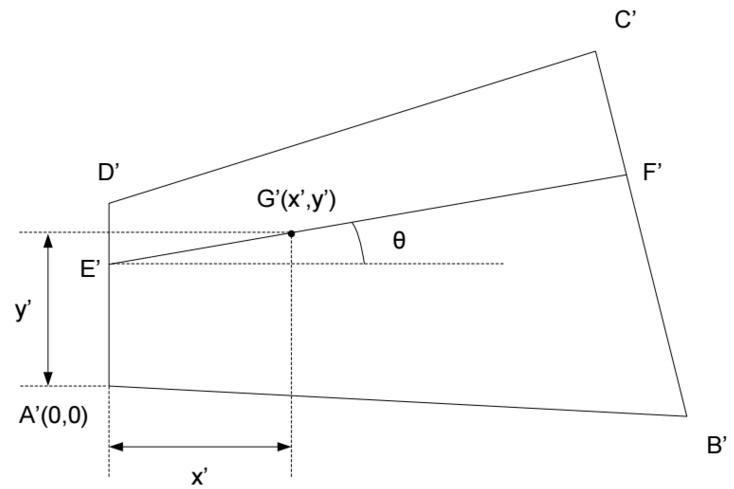
\includegraphics[width=0.45\textwidth]{figuras/retangulo00.jpg}\label{fig:f1}}
  \hfill
  \subfloat[retângulo]{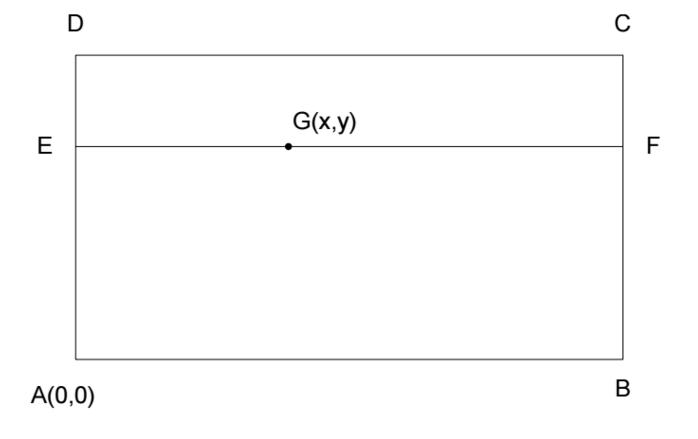
\includegraphics[width=0.45\textwidth]{figuras/retangulo01.jpg}\label{fig:f2}}
  \caption{transformação da região retangular A'B'C'D' no retângulo ABCD. Adaptado de \cite{inspect}.}
  \label{redimens}
\end{figure} 

%figura de: Kastelan, I., Katona, M., Marijan, D., & Zloh, J. (2011). Automated optical inspection system for digital TV sets. EURASIP Journal on Advances in Signal Processing, 2011(1), 1-17.

Dado que o retângulo transformado tem tamanho $(col_r,lin_r)$, que a região da imagem $A’B’C’D’$ é delimitada pelos pontos $A’ = (x_{a’},y_{a’})$, $B’ = (x_{b’},y_{b’})$, $C’ = (x_{c’},y_{c’})$ e $D’ = (x_{d’},y_{d’})$, podemos definir as variações dependentes de $x$ como $dx1 = \frac{x_{b’}-x_{a’}}{col_r}$ e $dy1 = \frac{y_{b’}-y_{a’}}{col_r}$. As variações dependentes de $y$ são $dx2 = \frac{x_{c’}-x_{a’}}{lin_r}$ e $dy2 = \frac{y_{c’}-y_{a’}}{lin_r}$.


Assim, um ponto $G(x,y)$ no retângulo transformado tem valores iguais a um ponto $G’(x’,y’)$ na imagem, segundo as equações:

$$ x = y_{a’} + dy1(x’) + dy2(y’) $$

$$ y = x_{a’} + dx1(x’) + dx2(y’) $$

O redimensionamento visa dar à imagem da tela o tamanho de uma imagem de referência, preparando-a para ser comparada com as imagens de referência. Esta é uma etapa necessária, como pode ser visto na subseção que fala das métricas de desempenho. Ele é feito através da interpolação bilinear, que é uma técnica de interpolação de funções de duas variáveis, o que a faz muito interessante para interpolar imagens.
Ela funciona interpolando linearmente as funções em uma direção e depois em outra. Supondo que se queira saber o valor da imagem na posição $I(x,y)$ e sabidos os valores nas posições $I(x_1,y_1)$, $I(x_1,y_2)$, $I(x_2,y_1)$ e $I(x_2,y_2)$, é encontrado o valor aproximado da imagem interpolando primeiramente no eixo $x$ através das equações:

$$ I(x,y_1) = \frac{x_2-x}{x_2-x_1}I(x_1,y_1) + \frac{x-x_1}{x_2-x_1}I(x_2,y_1) $$

$$ I(x,y_2) = \frac{x_2-x}{x_2-x_1}I(x_1,y_2) + \frac{x-x_1}{x_2-x_1}I(x_2,y_2) $$


E, após isso, interpolar os valores encontrados no eixo $y$, através da equação:

$$ I(x,y) = \frac{y_2-y}{y_2-y_1}I(x,y_1) + \frac{y-y_1}{y_2-y_1}I(x,y_2)$$

Com esta técnica, é possível obter uma aproximação do trecho da tela da TV ou monitor presentes na imagem capturada, do tamanho e formato necessários para a avaliação de desempenho.

\section{Métricas de Desempenho}

Este método utiliza três técnicas para avaliar seu desempenho em selecionar acertadamente o trecho da imagem que representa a tela. Estas técnicas comparam a imagem obtida, após rotacionada e redimensionada, com uma imagem de referência de mesmo formato e tamanho. Elas são:
\begin{itemize}
\item LAE (Least Average Error)
\end{itemize}



%LAE

O método LAE divide a imagem de teste e a de referência em regiões consideradas atômicas. Ele compara cada região na imagem de teste com a região correspondente na imagem de referência, portanto necessitando que as duas imagens tenham o mesmo tamanho e formato. Diferenças na iluminação entre as imagens comparadas podem resultar em valores de intensidade diferentes para a imagem, mesmo representando o mesmo objeto ou a mesma região. A fim de reduzir esta diferença, primeiramente as imagens são normalizadas utilizando a normalização estatística padrão. Dada uma imagem $A$, sua média $\mu_A$ e seu desvio padrão $\sigma_A$ são calculados e a imagem normalizada $A_n$ é dada pela equação \ref{normal}:

\begin{equation}
A_n = \frac{A-\mu_A}{\sigma_A} \label{normal}
\end{equation}

Assim, a média e o desvio padrão são calculados pixel a pixel para cada um dos três canais da imagem (R, G e B) e suas dessimilaridades são computadas e acumuladas, segundo a equação \ref{lae}:

\begin{equation}
D = \sum_ {x,y}^{} \sum_{c=R,G,B}^{} \left | \frac{A(x,y)-\mu _A}{\sigma _A} - \frac{B(x,y)-\mu _B}{\sigma _B} \right |
\label{lae}
\end{equation}

\begin{itemize}
\item NCC (Normalized Cross-Correlation)
\end{itemize}

O método NCC é baseado na correlação cruzada para medir a similaridade entre duas imagens. Assim como no LAE, para diminuir erros devido à diferença de iluminação, primeiramente as imagens são submetidas à normalização estatística padrão. A similaridade entre imagens normalizadas $A_n$ e $B_n$ é calculada segundo a equação \ref{ncc1}:

\begin{equation}
S = \iint A_n(x,y)*B_n(x,y) dx dy \label{ncc1} 
\end{equation}

ou, na forma discreta:

\begin{equation}
S = \sum \sum A_n(x,y)B_n(x,y) \label{ncc2} 
\end{equation} 


Sendo uma imagem normalizada segundo a equação:

\begin{equation}
A_n = \frac {A(x,y) - \mu_A}{\sqrt {\frac{1}{N}(\sum \sum {A(x,y)-\mu_A})^2}} \label{ncc3} 
\end{equation} 

em que $N$ é o número de pixels da imagem $A$, podemos calcular a similaridade entre duas imagens $A$ e $B$ segundo a equação \ref{ncc4}:

\begin{equation}
S = \frac{\sum \sum (A(x,y)-\mu _A)(B(x,y)-\mu _B)}{\sqrt{\sum \sum (A(x,y)-\mu _A)^2}\sqrt{\sum \sum (B(x,y)-\mu _B)^2}}
\label{ncc4}
\end{equation}

\begin{itemize}
\item NCC-BB (Normalized Cross-Correlation using Blocks)
\end{itemize}

Este método foi criado para contornar um problema encontrado pelo método NCC: sua pontuação depende do conteúdo da imagem, portanto tornando difícil a tarefa de escolher um limiar de similaridade que respondesse bem a qualquer imagem. Nele, é calculada a similaridade relativa entre as imagens.
Para isto são executados os seguintes passos:
\begin{itemize}
\item As imagens a ser comparadas são divididas em um $n$ blocos menores de mesmo tamanho;
\item É calculada a correlação cruzada da imagem de referência com uma imagem considerada correta para cada um dos blocos. Estes valores de similaridade são então guardados como um conjunto de valores padrão $S_{padrao}$;
\item Para cada imagem de teste submetida ao método, é calculada a correlação cruzada em cada um dos seus blocos;
\item Os valores de similaridade encontrados são comparados bloco a bloco e somados para compor o valor de similaridade relativa. Sendo $S_{A,B}$ a similaridade entre as imagens $A$ e $B$, a similaridade relativa pode ser calculada através da equação \ref{nccbb}

\begin{equation}
S = \max_{blocos}|S_{A,B} - S_{padrao}| \label{nccbb}
\end{equation}

\end{itemize}
%cada imagem é dividida em um $n$ blocos menores e é computada a correlação cruzada em cada um destes blocos, ao invés de na imagem toda. Primeiramente, a imagem de referência é dividida nestes blocos e é calculada a sua similaridade com uma imagem considerada correta. Estes valores de similaridade são então guardados como um conjunto de valores padrão $S_{padrao}$.
%Após isto, para cada imagem de teste submetida ao método, é feito o cálculo da similaridade em cada um dos seus blocos e os valores são comparados com os encontrados em cada região e somados para compor o valor de similaridade relativa. Sendo $S_{A,B}$ a similaridade entre as imagens $A$ e $B$, a similaridade relativa pode ser calculada através da equação \ref{nccbb}

%\begin{equation}
%S = \max_{blocos}|S_{A,B} - S_{padrao}| \label{nccbb}
%\end{equation}